\chapter{Research Plan}
This chapter will present the research project. Specifically, the discussion will begin with a description of the various research gaps that can be extrapolated from the current literature and the importance of addressing these gaps with respect to the ultimate goals of Learning from Demonstration. Next, the research proposal for the next two years will be presented, contextualizing it within the previous study and highlighting its strengths and importance. Along with the presentation of the project, the techniques and methodologies used to implement the project and evaluate the results obtained will also be described.

\section{Research Topic}
\label{sec:research_topic}
\todo[inline]{Organizzazione logica sequenziale. Contesto e problemi della robotica classica rispetto alle nuove applicazioni. Introduzione dei metodi di interesse. Osservazioni riguardanti i metodi di interesse. Giustificazione degli errori. Proposta, risponde alle domande cosa, come e perché. Tutto con attenzione ai termini utilizzati, frasi semplici e chiare, accompagnate da esempi.}
% General descritpion
One of the primary objectives in robotics is to develop autonomous robots capable of performing a wide range of manipulation tasks, such as pick-and-place and assembly operations, in response to specific commands. These tasks are often characterized by some degrees of variability, which may be related to factors like object categories and positions.
\newline In the context of traditional industrial operations, \hl{manually coded control rules can effectively manage situations in which robots follow fixed and repetitive paths. This is achieved through prior knowledge of object categories and positions, within an environment where the robot's working area is known and fixed over time} \change{\small Termini chiari e semplici. Facile capire il problema dei metodi classici} (e.g., the workcell in Figure \ref{fig:industrial_robots_example}).
In contrast to this scenario, the contemporary landscape of social robotics and modern industrial applications demands a higher level of adaptability and flexibility. Robots are expected to work in environments alongside human operators, receiving commands and engaging in interactions with them in a collaborative or cooperative manner. For example, a robot may be tasked with picking up a tool and delivering it to the operator. This entails the robots' ability to recognize various object categories and estimate their positions but also correlate the outcomes of environmental analysis with the requested commands and adapt their actions accordling, showing ``intellingent'' behaviors.

% Introduction to target methods
As extensively discussed in Chapter \ref{chapter:background}, the scientific community has directed its attention towards addressing these challenges by evaluating the utilization of \textit{data-driven} approaches. These methods encompass Imitation Learning algorithms, which utilize data derived from examples of desired behaviors, often referred to as demonstrations, to equip a robot with the capability to replicate the demonstrated tasks.
\change{\small Multi-Task: Perché, Come funziona, Concetti essenziali per la comprensione}
\newline Multi-Task Imitation Learning methods, as highlighted in \cite{jang2022bc_z, dasari2021transformers_one_shot, mandi2022towards_more_generalizable_one_shot, brohan2022rt}, are notably promising due to their capacity to fulfill the requirements of both high \textit{adaptability} and \textit{flexibility}. As extensively explained in Section \ref{sec:methods}, these methods use a \textbf{multi-task dataset} $\mathcal{D}^{E} = \left \{ \mathcal{D}_{1}, \dots \mathcal{D}_{n}\right \}$, which contains demonstrations for $n$ different tasks (e.g., $\mathcal{D}_{1}$ contains demonstrations of pick-place task, $\mathcal{D}_{2}$ contains demonstrations of nut-assembly task and so forth), to fit a \textit{single control function} denoted as $\pi^{L}_{\theta}(a_{t}|s_{t}, c_{m_{i}})$, that is able to map the current observed state $s_{t}$ and the command $c_{m_{i}}$, into the corresponding action $a_{t}$ that will be executed by a phisical robot. The command $c_{m_{i}}$ referes to the $m^{th}$ variation of the $i^{th}$ task (e.g., the pick-place task can have different variations based on the target object and the target placing spot as depicted in Figure \ref{fig:mosaic_tasks}). Tables \ref{table:mosaic} and \ref{table:rt1_results} illustrate the potential of the proposed approaches, yet challenges remain in both single-task and multi-task problems. As reported in \cite{jang2022bc_z, yu2018daml}, existing systems face difficulties in \hl{identifying critical task} \change{\small Errori dei metodi, spiegato cosa sono i critical point, cosa sono i distractor objects} \hl{points, such as determining when to close the gripper near an object or open it in proximity to the placement area}, rather than understanding the broader intent of the task at hand. Furthermore, performance drops occur when scenes involve distractor objects, i.e.,  objects  that  do  not  contribute  to  the  task  execution. This highlights the need for improved capabilities in correctly correlating commands with the results of scene analysis to identify target objects.

% Propose research activity
In the context presented so far, this research activity aims to address the problem of \textit{Learning from Demonstration} in multi-task scenarios. Our aim is to develop a system that can make a step towards the realization of a \hl{\textit{versatile \ collaborative \ robot} suitable for industrial applications. This robot should possess the capability to execute tasks directed by a human operator and acquire new skills based on a limited number of demonstrations, building upon its existing knowledge. To illustrate potential applications, consider a collaborative workspace where a human operator could instruct the robot to provide a tool or engage in assembly tasks}.
\change{\small Goal industriale con esempio}
\newline With respect to the general formulation extensively explained in Section \ref{sec:methods}, we are interested in exploring methods that rely on \hl{\textit{visual \ inputs}, i.e., the current state $s_{t}$ is an image that depicts the current state of robot workspace, and the command $c_{m_{i}}$ is given in terms of video demonstrations of an agent (e.g., robot or human) that executes the desired task}.
\change{\small Nostro sistema, qual è l'input?}
\newline In addition to the overall assessment we conducted following the literature review, it is essential to emphasize that significant modifications have been made in relation to the Research Proposal presented at the conclusion of the first year. These alterations were prompted by interesting insights obtained from preliminary experiments, which subsequently enabled us to identify a previously unexplored research gap and formulate the ensuing research question:
\paragraph{\textit{Reason-then-act: How the separation between perception and action can affect the performance of an Imitation-Learning System}} \mbox{} \\
In both \textit{``Language-Conditioned Imitation Learning"} and \textit{``Video-Conditioned Imitation Learning"}, the primary objective is to obtain a function $\pi_{\theta}^{L}$, that can effectively map the current state and command pair to the corresponding action. These systems need to address two key challenges:
\begin{enumerate}
    \item \hl{\textbf{Command \ analysis \ and \ understanding}}\change{\small Utilizzo di termini più appropriati}: The first challenge involves the
          analysis of the given command. Specifically, from an \textbf{high-level task command} the system should be able to understand the \hl{\textbf{intent} (e.g., picking and placing rather than assembling), identify the relevant objects (e.g., selecting the blue box rather than the red one), and recognize the mentioned actions (e.g., reach, follow, pick)}\change{\small Esempi per facilitare la comprensione}. In language-conditioned systems, neural language models \cite{stepputtis2020language,jang2022bc_z,brohan2022rt}, are commonly employed to extract and represent the semantics of the command. In image-conditioned systems, image processing and computer vision techniques (e.g., deep learning architectures \cite{dasari2021transformers_one_shot,mandi2022towards_more_generalizable_one_shot}) are used to extract relevant features from the video demonstration.
    \item \textbf{Action Generation}: The second challenge is to correlate the features generated from the analysis of the observed state and the information obtained from the command, with the aim to create an intermediate representation that captures the relevant aspects from both inputs (e.g., there is a focus on the image portion that contains the target object). Techniques such as feature concatenation \cite{james2018task_embedded,stepputtis2020language,bhutani2022attentive_one_shot}, attention mechanisms \cite{dasari2021transformers_one_shot,mandi2022towards_more_generalizable_one_shot}, or feature-wise linear modulation \cite{brohan2022rt} are utilized to combine the visual information from the state and the information from the command. The fused representation should capture the important cues for inferring the correct action based on the current input and command.
\end{enumerate}
Despite the progress made with Multi-Task Imitation Learning, the performance of these agents still lacks consistent robustness when faced with challenges such as distractor objects and varying backgrounds \cite{brohan2022rt}. During our preliminary experiments (Chapter \ref{chapter:preliminary_results}) we tried to emphasize this problem in order to \textbf{focus our attention to scene analysis and cognitive aspects} rather than pure control problems, by testing the models in scenarios where there are objects that differ in very high-level features such as the color. Indeed, our preliminary experiments revealed a noteworthy observation. \hl{While our system consistently generates what can be referred to as ``valid trajectories", i.e., it effectively carries out the actions of picking up an object and correctly placing it in the intended position, it often struggles with the critical task of identifying the precise target object. In other words, there is a recurrent issue where the selected object for manipulation is not the correct one}\change{\small Osservazioni chiare e precise}.
\newline The observed results can be explained through a comprehensive analysis of the underlying learning procedure. Specifically, the reference methods \cite{dasari2021transformers_one_shot,mandi2022towards_more_generalizable_one_shot,brohan2022rt} propose end-to-end architectures that starting from \textbf{high-level inputs} (e.g., images and text) directly generate the required action, assuming that there is an implicit solution to the initial challenges associated with the command analysis and comprehension. These architectures are trained based on the principles of Behavioral Cloning (BC). BC offers two main approaches: one involves minimizing the disparity between the predicted and correct actions (as shown in Formula \ref{eq:mse}), while the other centers on maximizing the likelihood of executing the correct action (as shown in Formula \ref{eq:nll}). The choice between these approaches hinges on the nature of the policy, whether deterministic or probabilistic. It's important to note that all of these loss functions primarily target the predicted action, directly addressing step 2, with an implicit assumption of resolving step 1. This approach has exhibited effectiveness in simple scenarios where the robot has to learn a single task without variations \cite{zhang2018deep_vr_teleoperation,duan2017one_shot_il} and in multi-task settings where scenes are comprised of easily distinguishable objects \cite{dasari2021transformers_one_shot,mandi2022towards_more_generalizable_one_shot,brohan2022rt}. However, in complex scenarios composed of different distractor objects, the cognitive task becomes considerably more intricate and may be beyond resolution solely through the information derived from the action-based loss, increasing the gap that exists between the training metric and the actual goal (i.e., understand the command, genarete the action based on the current state and the command comprehension, and solve the desired task).
Starting from all the considerations above, the stated problem can be faced in two ways:
\begin{enumerate*}[label=(\arabic*)]
    \item Enhancing dataset diversity by expanding the representation of objects and employing a large-scale model capable of assimilating all the knowledge inherent in the dataset.
    \item Dividing the Decision-Making Problem into two primary blocks, namely a reasoning module and an action module. This segmentation enables the independent validation of each task within the decision-making process and the separate evaluation of the performance of each block. Subsequently, a method should be devised to integrate these two components, creating a modular system capable of solving complex problems. This system would consist of interconnected modules designed to address simpler problems.
\end{enumerate*}
In our second year of research, we opted to concentrate on a procedure aligned with the second approach. This choice was motivated by its effectiveness in assessing the various sub-tasks inherent in a decision-making problem, such as the control of a robotic system. Comprehensive details regarding the exact procedure and its formalization will be presented in the forthcoming Section \ref{sec:research_activity}.

\section{Proposed Research Activity}
\label{sec:research_activity}
After the presentation of the context of interest and the aspects to be treated in the current research proposal, this section will formalize the improvement hypotheses reported in Section \ref{sec:research_topic}, identifying the main methods of interest from which will start the application of the proposed changes, and the procedures that will be used to validate and compare the proposed approach against the state-of-the-art methods.
Starting from the discussion made in Section \ref{sec:research_topic}, one consideration arises. Given a scenario where the robot must execute a task given a command, how to model a system that is able to identify the objects of interest, which may change based on the command.
In literature, there are recent \textit{Imitation Learning methods}, that follow an object-oriented paradigm \cite{park2021object, belkhale2023plato, zhu2023viola, jiang2023vima}. However, methods like \cite{belkhale2023plato} primarily focus on learning the affordance of individual objects. These methods take as input the current observation and the desired state of a specific object, typically in single-object scenarios. On the other hand, techniques in the field of Vision-Based Manipulation, such as \cite{zhu2023viola, jiang2023vima}, leverage pre-trained object detectors like Mask-RCNN \cite{he2017mask}. These detectors identify the top-k predicted bounding-boxes that \textbf{potentially contain objects} in the scene and utilize this information to infer the appropriate actions. In contrast to these methods, our approach draws inspiration from Computer Vision tasks like 'Vision Question and Answering' \cite{perez2018film}. In this task, the system is responsible for generating an answer to a given query (e.g., a textual representation of a question) based on an input image. What distinguishes this approach is its capability to \textbf{selectively focus on specific segments of the image}, guided by the content of the question, as illustrated in Figure \ref{fig:film_attention}
\begin{figure}[htb]
    \centering
    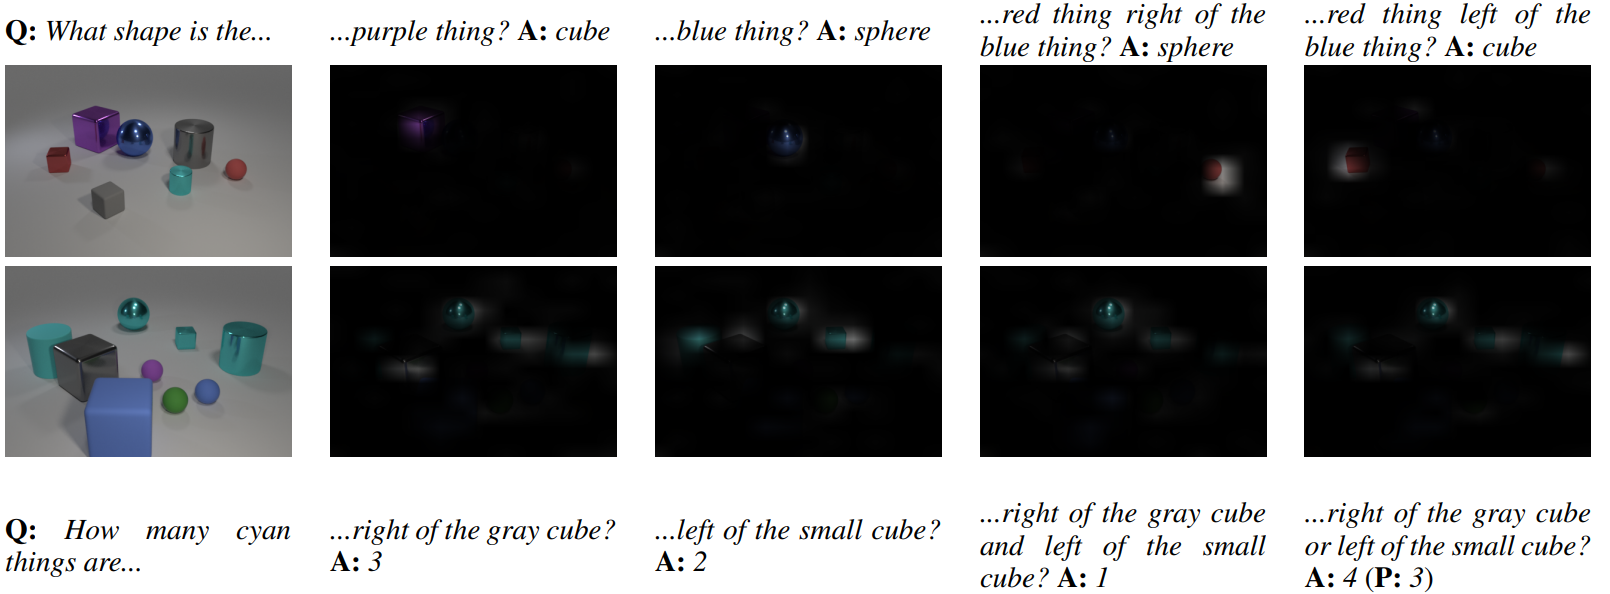
\includegraphics[width=0.9\textwidth]{Figures/images/film/film_attention.png}
    \caption{\textit{Vision Question and Answering task}, starting from a an image and a text, the method is able to generate an answer by focusing on specific part of the image based on the question.}
    \label{fig:film_attention}
\end{figure}

In conclusion, our research focuses on evaluating the adaptability of visual-scene reasoning modules, as exemplified by \cite{perez2018film}, to address a novel problem termed \textit{`Conditioned-Target Object Detector'}. The primary objective is to develop a system capable of precisely identifying a the \textit{\textbf{target object}} based on the desired task. This kind of problem can be formulated as an \textbf{\textit{Object Detection Problem}}, as it will be formulated in Chapter \ref{chapter:preliminary_results}. Moreover, in a multi-task context, such a system needs to be \textit{\textbf{object-class agnostic}}, meaning it should have the ability to predict both box-shaped target objects and nut-shaped target objects without any prior knowledge about the object's class.
In order to validate the hypothesis that following a modular approach can affect positively the system performance, we will follow an incremental approach, divided into 4 main steps:
\begin{itemize}
    \item \textbf{Baseline Definition}: This initial step is crucial to establish a baseline and pinpoint critical aspects of the current state-of-the-art methods
    \item \textbf{Incorporate Ground-Truth Information into the Baseline's Control Module}: After assessing the baseline, the second phase focuses on empirically assessing whether adding target-object information to the control modules can enhance system performance. During this phase, to prevent error propagation, the control module will receive input based on ground-truth information.
    \item \textbf{ Development of a Conditioned-Target Object Detector System}: Once the second step is completed, we can formulate the Conditioned-Target Object Detector problem and evaluate its efficacy in addressing the tasks at hand.
    \item \textbf{Integration of the Developed System with the Baseline}: After achieving a stable system in the previous step, we will integrate the developed system with the baseline architecture to assess overall system performance
\end{itemize}
In the initial iteration, the methods will undergo training in a Single-Task Multi-Variation scenario. Subsequently, leveraging the class-agnostic property, the system will be extended to a Multi-Task Multi-Variation setup.
Results and additional details concerning these problems will be presented in Chapter \ref{chapter:preliminary_results}."
% \newline As discussed in Section \ref{sec:research_topic}, it was seen that current methods start from a representation of the environment that lacks geometric information and that is obtained from the point of view different from that of the robot, and in particular from that of the end-effector. 
% Concerning this point, starting from the state-of-the-art architecture \cite{mandi2022towards_more_generalizable_one_shot} based on Transformer, the goal will be to extend it in such a way that it will be able to handle time sequences characterized by RGB-D observations, and taken from a camera mounted on the end-effector. Several approaches can be used to achieve this. In fact, in the Computer Vision community, RGB-D images can be handled in different ways. For example, one can apply convolutional layers separately on the RGB and depth images, as in \cite{zhang2018deep_vr_teleoperation}, and subsequently perform a fusion between the extracted features based, for example, on their concatenation. Another approach may be using a 3D Point-Cloud Neural Network, such as \cite{qi2017pointnet++} used in \cite{fang2020graspnet}. To answer the question which of the two approaches to prefer, given that the reference method \cite{mandi2022towards_more_generalizable_one_shot} has a transformer-based architecture, a first step may be to apply convolutional filters separately on the RGB and D images and then combine them appropriately, going on to evaluate different fusion techniques, starting from simple concatenation to the use of a weighted sum, with the ultimate goal of generating the embedding as input to the transformer.
% \newline This setting will allow evaluating the hypothesis that adding geometric information can reduce failures caused by collisions with objects of interest or by the inability to determine when to close or open the gripper.  
% The resulting method will then be tested and compared first in simulation, taking advantage of the open-source simulation environments \cite{brockman2016openai,zhu2020robosuite}. Then, based on the obtained results, the proposed architecture will be tested and evaluated on a real robot platform, adding an additional experimental contribution that current methods such as \cite{dasari2021transformers_one_shot,mandi2022towards_more_generalizable_one_shot} lack.
% \newline As for the tasks of interest, the main focus will be devoted to industrial tasks (e.g., pick-and-place, push, peg-insertion), introducing an additional constraint with respect to \cite{mandi2022towards_more_generalizable_one_shot}, since the system will have to be able to perform real-time inference on low-cost embedded platforms, in order to control a real-world robot platform.
% \newline An incremental approach will be used for the design and development of the proposed system. Thus, a single-task setting will first be evaluated, but, with respect to \cite{mandi2022towards_more_generalizable_one_shot}, it will be characterized by a high degree of variability based on different initial conditions and different objects to be manipulated so as to evaluate the ability to generalize across a single task, a setting in which meta-learning-based procedures have proven successful \cite{finn2017one_shot_visual_il,yu2018daml}. Next, the system will be extended into a multi-task context, where the hypotheses made earlier about using Variational-Autoencoder for learning a representation related to the demonstrated sub-tasks can be evaluated and validated in combinations with the use of Contrastive Loss, which have been shown to be valid in methods such as \cite{sermanet2018time_contrastive,zakka2022xirl} where the goal has been to learn a task representation from different embodiments \cite{zakka2022xirl} and different viewpoints \cite{sermanet2018time_contrastive}. Here, with respect to \cite{Mandlekar2020GTI}, the Variational Autoencoder will be combined with Contrastive Loss, to learn a sub-task related representation starting from demonstrations composed of different visual appearance. While, with respect to \cite{mandi2022towards_more_generalizable_one_shot}, the proposed combination aims to model explicitly the concept of sub-tasks, which may help the generalization in a multi-task settings by leveraging the task hierarchical structure.

Based on the State of the Art, presented in Chapter \ref{sec:sota}, the following research-gaps can be identified ...., and the following questions can be made...